\documentclass{article}

% Language setting
% Replace `english' with e.g. `spanish' to change the document language
\usepackage[english]{babel}

% Set page sise and margins
% Replace `letterpaper' with `a4paper' for UK/EU standard sise
\usepackage[letterpaper,top=2cm,bottom=2cm,left=3cm,right=3cm,marginparwidth=1.75cm]{geometry}

% Useful packages
\usepackage{amsmath}
\usepackage{graphicx}
\usepackage{parskip}
\usepackage[colorlinks=true, allcolors=blue]{hyperref}

\title{The Automation of Artistry: The Applications and Ethical Implications of Generative AI in Music}
\author{Alex Manning}

\begin{document}
\maketitle

\section{Introduction}
Generative AI music tools have gone from research prototypes to commercially available platforms in less than two years. You can now generate a song as easily as you would generate an image or a paragraph of text. This rapid advancement raises profound ethical, legal, and cultural questions. Who owns music created by machines trained on human works? Can such music be protected under copyright law? And what happens to musical diversity and authenticity when algorithms start to shape the musical landscape?

This essay examines the rise of generative AI music through four lenses: the technological developments that made it possible and its current applications, the legal and ethical crises surrounding data use and authorship, the cultural implications for Māori data sovereignty, and the evolving consumer attitudes that will shape the future of this technology. Together, these sections argue that while AI music systems possess extraordinary technical power, their integration into society must be guided by strong ethical frameworks, transparent governance, and a commitment to human creativity.

\section{The New Landscape}

Generative AI music systems have seen a sudden acceleration in development and capability after decades of gradual improvement. Early algorithmic composition systems, such as the Illiac Suite in the 1950s, used rule-based approaches like Markov chains to generate musical scores \cite{funk2018musical}. Through the late 20th and early 21st centuries, development remained largely academic, progressing through neural network experiments with symbolic MIDI generation, such as MusicVAE \cite{roberts2018hierarchical} and direct audio synthesis, such as AudioLM \cite{borsos2023audiolm}. These early systems produced musically incoherent results, lacking the structural coherence and audio fidelity needed for practical application.

[Audio of Illiac Suite]
[Audio of MusicVAE]
[Audio of AudioLM]

The technical innovation that enabled current generative music systems was the application of transformer architectures to audio. Google's MusicLM \cite{agostinelli2023musiclm} demonstrated that by tokenising audio and text into a shared latent space, models could generate structurally coherent music from text prompts, maintaining consistent genre, rhythm, and instrumentation across extended durations. A parallel development in diffusion models, which reconstructs audio by iteratively denoising random noise, further improved output quality. Systems like Noise2Music \cite{huang2023noise2music} and Riffusion \cite{coldewey2022riffusion} applied this approach by generating spectrograms and converting them into audio waveforms. The combination of transformer-based structural coherence and diffusion-based audio quality produced the first systems capable of generating commercially viable music from text prompts.

[MusicLM Adudio]

The gap between academic research and commercial deployment for this technology was brief. Suno launched in December 2023 \cite{sunoai}, followed by Udio in April 2024 \cite{udio}. Both platforms translated complex generative models into accessible web interfaces, making high-fidelity song generation available to any user. This rapid commercialisation established prompt-to-song generation as a widely accessible technology.

The primary commercial application of generative AI music so far has been in utility contexts: background music for content creation, ambient soundscapes, and advertising, where the music functions as a tool rather than as artistic expression \cite{stammer2024generative}. Platforms like Canva, Soundful, and Filmora have integrated AI music generation directly into their content creation workflows, allowing users to generate royalty-free background tracks without having to navigate traditional music licensing. On YouTube, AI-generated ``focus music" and lo-fi hip-hop channels regularly accumulate hundreds of thousands of views, serving listeners who desire unobtrusive audio for studying or working. With this type of music the listener's relationship to it is purely transactional, the music exists to fulfill a specific atmospheric or legal need.

[insert youtube lofi ai music add highlight how many views it has]

Beyond this built for utility music, generative AI has recently started being used to create synthetic artists with constructed identities and brands. In mid-2025, The Velvet Sundown, a band later revealed to be entirely AI-generated, accumulated over 1.4 million monthly Spotify listeners before publicly confirming that its music, vocals, and visuals were created using AI \cite{berklee2025velvet}. The project, framed by its creators as an ``artistic provocation," initially fooled major publications including Rolling Stone, which published interviews with a fabricated spokesperson. Similarly, AI musician Xania Monet, created by songwriter Telisha Jones using Suno, secured a \$3 million record deal after generating 9.8 million streams and achieving a No. 1 position on Billboard's R\&B Digital Song Sales chart \cite{petraeus2025goodbye}. However, other major labels reportedly declined to bid on Monet because of ongoing copyright litigation against Suno. These cases demonstrate that AI-generated music can achieve commercial success when packaged with artist personas and marketing, though they also expose the risk of AI music as it currently stands, as major industry players remain hesitant to invest in AI artists while the legal status of their training data remains unresolved. It should also be noted that while these artists have accumulated millions of streams, public reception has been mixed at best, with significant push back from listeners who refuse to consider AI-generated output as legitimate art.

[insert youtube video of a velvet sundown song]

\section{The Ethical and Legal Crises}

The rapid commercialisation of generative AI music has outpaced the development of appropriate legislation and ethical guidelines. While the previous section documented what AI music systems can do and how they are being deployed currently, this section examines whether their current implementation is legal or ethical, and what regulatory measures may be needed. Three main issues are at play here: whether AI companies are legally permitted to use copyrighted music as training data without compensation, whether AI-generated music itself warrants copyright protection, and whether the practice of training models on AI-generated output risks degrading the quality and diversity of future musical output. 

\subsection{Training Data Concerns}
Companies like Suno and Udio require enormous datasets to train their generative AI models effectively. Unlike traditional Text and Data Mining systems (TDM) that extract patterns and knowledge, generative AI models aim to approximate the probability distribution of their training data to produce outputs that mimic the structure and style of the original material. These companies have scraped virtually all accessible music from the internet to build datasets large enough to generate high-quality, diverse musical outputs. The scale and means of data collection creates legal and ethical questions about consent, compensation, and the rights of original musicians.

Both Suno and Udio claim their use of copyrighted music falls under ``fair use" protections. However, recent legal discussion challenges this position. A 2025 paper \cite{dornis2025generative} argues that the legal landscape for training generative AI with copyrighted material is currently fragmented and uncertain, and that existing copyright exceptions may not apply to generative AI training due to its fundamentally different purpose compared to traditional TDM. The International Confederation of Societies of Authors and Composers (CISAC), representing over 5 million creators globally, also argues that AI companies scrape copyrighted content without permission, incentivised by the direct relationship between training data quality and model performance \cite{cisac2023statement}.

These concerns have materialised into multiple lawsuits. In 2024, the Recording Industry Association of America (RIAA), representing major labels including Sony Music, UMG, and Warner Records, filed copyright infringement suits against both companies for ``mass infringement" through unauthorised copying of sound recordings, arguing that their outputs constitute ``imitative machine-generated music, not human creativity or expression" \cite{connelly2024record}. More recently, independent artists filed additional lawsuits in Illinois accusing Suno and Udio of obtaining copyrighted recordings through ``stream-ripping" from YouTube and scraping lyrics from databases like Genius and AZLyrics without licenses, alleging the companies maintain internal libraries of copied files without proper deletion protocols \cite{dalugdug2024suno}. These independent artists argue the AI models create ``competitive, radio-quality substitutes" that reduce demand for their work and decrease licensing opportunities, causing direct market harm to creators who can least afford it.

Generative AI does not fit within current copyright law due to its capability to use training data to replicate the art present in this data. Even if these companies currently operate in a legal grey area, recent court proceedings indicate that new generative AI legislation will likely require explicit permission from creators and musicians to train on their work. This would be the correct outcome from an ethical standpoint as the current arrangement violates the common good by using musicians' art against their will to train models that then create music to directly compete with those same human artists, funneling wealth to a small number of AI companies and away from the musicians whose creativity and innovation formed the foundation upon which these models operate.

\subsection{Is AI Music Copyrightable?}
Copyright law exists to incentivise human creativity by granting authors exclusive rights to control and profit from their work. In the United States, the Copyright Act of 1976 protects ``original works of authorship fixed in any tangible medium of expression" for the life of the author plus 70 years, while New Zealand's Copyright Act 1994 provides similar protection. These laws were designed around the assumption that creation is a human act, an expression of individual perspective, skill, and intention.

Extending copyright protection to purely AI-generated music would be a net negative for the music industry. Streaming platforms, record labels, and distributors will be incentivised to flood the market with AI music rather than invest in human musicians. AI-generated content is cheaper to produce, infinitely scalable, and requires no ongoing artist relationships, royalty negotiations, or touring support. The Authors Guild, in opposing copyright protection for AI-generated text, argues that allowing such protection would enable ``homogenised mashups" to compete with and displace human-authored work, shrinking the profession and ``shutting out diverse voices" \cite{authorsguild_ai}. Without restrictions limiting generative AI's ability to be monetised the resulting artistic output will decline in quality and diversity. This applies directly to music: if labels can copyright AI-generated albums at a fraction of the cost of human recording contracts, the economic pressure to replace human rosters becomes overwhelming. The music industry would face the same market dilution the publishing industry is seeing.

Recent regulatory developments in the United States have clarified that generative AI outputs do not meet the threshold for copyright protection when created solely through prompts. In January 2025, the U.S. Copyright Office released Part 2 of its Report on AI and copyright, concluding that ``the outputs of generative AI can be protected by copyright only where a human author has determined sufficient expressive elements" \cite{usco_newsnet_1060}. The Office explicitly stated that ``the mere provision of prompts is not enough to secure copyright." This position was legally affirmed in Thaler v. Perlmutter, where the D.C. Circuit Court ruled that Dr. Stephen Thaler could not copyright an artwork created by his AI system \cite{cadc_2025_23_5233}. The Court's reasoning emphasised that the Copyright Act's structure, including provisions for author lifespan, inheritance, and intention, presumes human authorship. As the Court noted, computer programs are defined as ``tools used by humans to assist authors, not as authors themselves." The ruling does not prevent copyrighting works made with AI assistance, only works where the machine's output constitutes the sole creative contribution. This legal framework, if applied to music, would allow copyright protection for compositions where AI serves as a tool within a larger creative process directed by human authors, but not for entirely prompt-generated songs.

New Zealand's legislation currently lags behind the United States on this issue. The Copyright Act 1994 does not explicitly address AI-generated works, leaving ambiguity about whether prompt-only creations could be granted copyright protection. Without clear legislation comparable to the U.S. Copyright Office's 2025 ruling, New Zealand risks incentivising the displacement of human musicians. However, even with updated legislation, enforcement will be difficult. AI-generated music is not always detectable, current detection tools produce false positives and can be circumvented through post-processing. More importantly, distinguishing between a purely prompt-generated song and legitimate AI-assisted human composition is messy. Consider this: a musician generates ten AI variations of a melody, picks one, modifies the arrangement, records live vocals over the top, and adjusts the mix, at what point does this constitute ``sufficient human expressive elements"?

\subsection{The Consequences of a Musical Model Collapse}

Current generative AI music models benefit from being trained exclusively on human-created music. Their datasets contain decades of genuine creative innovation, stylistic experimentation, and the productive accidents that define musical evolution. When the Beatles' ``I Feel Fine" opens with unintentional guitar feedback that became iconic, or when James Brown's drummer Clyde Stubblefield created the ``Funky Drummer" break through improvisation that would become the most sampled beat in history, these moments came from human error, spontaneity, and risk-taking. AI models trained on this rich history can mimic its patterns and produce convincing outputs. But these models don't replicate the creative accidents, they generalise. Ask for a country song and you get a track that sounds like the statistical average of country music: conventional chord progressions, predictable lyrical themes, familiar instrumentation. 

The problem gets worse when generation-two models train on datasets contaminated with AI-generated content. A 2024 study showed that AI models experience ``model collapse" when trained on recursively generated data \cite{shumailov2024collapse}. The models ``mis-perceive reality" and progressively lose information about the original data distribution, with unusual, boundary-pushing elements disappearing first. Over successive generations, outputs converge toward ``a point estimate with very small variance," producing results that have ``little resemblance to the original data." In an experiment with language models, sequential fine-tuning on model-generated text caused severe performance degradation, outputs became repetitive and nonsensical. Preserving 10\% of original human-generated data in each training cycle significantly reduced this collapse, proving how critical human creativity is to maintaining model quality.

For music, this trajectory is worrying. If streaming platforms and content libraries get flooded with AI-generated tracks, music that's already a generalisation of human creativity, the next generation of models will train on increasingly bland data. Over multiple iterations, musical diversity will reduce. Genre distinctions blur as models drift toward the statistical center of ``popular music," producing tracks that sound professionally made but culturally hollow. 

If AI-generated music is going to be part of our culture, AI companies have an ethical responsibility to prevent this homogenisation of music. Music's cultural role depends on its ability to reflect diverse human experiences, challenge conventions, and generate new aesthetic ideas. A homogenised musical landscape produced by recursive AI training would kill these aspects, turning it into an industrial commodity rather than a form of human expression.

\section{Aotearoa Case Study: AI, Tikanga, and Data Sovereignty}

As established in the Consequences of a Musical Model Collapse Section, AI music models generalise musical output toward statistical averages of their training data. This has particular implications for Indigenous music traditions, which are severely under-represented in the datasets used to train commercial generative AI systems. A 2024 analysis of existing music datasets found that only 5.7\% of total training data comes from non-Western genres, with the majority dedicated to Western music \cite{mehta2025music}. European, East Asian, and American music account for 84.5\% of available data, while South Asian, Middle Eastern, Central Asian, and African music each contribute less than 1\%. This imbalance leads to poor quality outputs when models attempt to generate non-Western music, often defaulting to Western tonal structures and instrumentation. For Māori music in Aotearoa, this data disparity means that generative AI systems like Suno and Udio have poor ability to authentically represent Māori musical traditions, which are built on fundamentally different structural principles, vocal techniques, and cultural contexts than the Western popular music that dominates their training sets.

This technical limitation raise questions of data sovereignty and tikanga Māori. The principle of kaitiakitanga (guardianship and stewardship over cultural taonga) requires that Māori maintain control over how their knowledge is collected, used, and represented, including musical traditions \cite{lilley2024maori}.Kaitiakitanga emphasises the protection and preservation of cultural resources for future generations, rooted in the interconnectedness of people, knowledge, and land. Current AI music systems operate in direct opposition to this principle. When AI models scrape publicly available recordings of Māori music without permission or cultural consultation, and then use that data to generate outputs that may misrepresent or dilute those traditions, there is no guardianship and no accountability to the communities whose culture is being commodified. The right of rangatiratanga (self-determination), guaranteed by Te Tiriti o Waitangi, includes the authority to exercise control over Māori data from collection to application \cite{lilley2024maori}. Yet AI companies have decided to train on whatever data they can access, with no means for Māori communities to consent to, benefit from, or correct the representation of their culture in these systems.

To illustrate this problem, AI music platform Suno was used to generate a Māori karanga. A karanga is a ceremonial call performed by women during pōwhiri (welcome ceremonies), used to establish spiritual connection between tangata whenua (hosts) and manuhiri (visitors). The karanga is a highly skilled practice with specific vocal techniques, structural patterns, and cultural protocols that vary between iwi (tribes). It carries whakapapa (genealogy), acknowledges tūpuna (ancestors), and fulfills a sacred role in the ritual process. 

[Audio: Authentic karanga] 
[Audio: AI-generated karanga] 

The AI-generated version was fundamentally flawed. It featured a male voice rather than female, included percussive elements, and incorporated major chord harmonies. These errors stem from Western-biased training data and result in output that is not only inaccurate but culturally inappropriate, bordering on a form of digital colonialism that misrepresents and distorts Indigenous practices.

Addressing these issues requires significant changes to how AI systems engage with Indigenous data and cultural knowledge. Research on incorporating Indigenous knowledge systems into AI governance suggests that frameworks must move beyond Western-centric models of individual data rights toward collective stewardship and relational accountability \cite{ray2024incorporating}. For Māori, this means applying tikanga principles throughout the AI development process. Kaitiakitanga would require AI companies to establish genuine partnerships with Māori communities, obtaining explicit permission before training on Māori musical data and providing mechanisms for ongoing oversight and correction. Whanaungatanga (relationship-building) requires sustained engagement rather than extractive data collection. Manaakitanga (reciprocity) requires that Māori communities be the primary beneficiaries of any AI systems trained on their cultural material, not merely data sources for commercial products. 

However, this raises a fundamental question: is it even possible to have AI-generated Māori music that aligns with tikanga? The karanga experiment suggests significant tensions. Māori music traditions are not simply sonic patterns to be replicated. They are vessels for whakapapa, mana, and cultural knowledge that exist within specific relational and ceremonial contexts. A karanga generated by an AI system has no whakapapa, no understanding of the ancestors it invokes, no awareness of the spiritual role it performs. It is a hollow imitation of form without substance. Even if technical quality improved dramatically, the question remains whether music separated from human intention can ever be considered legitimate within a tikanga framework. Perhaps the appropriate answer is not to make AI-generated Māori music ``better," but to recognise that some cultural practices should remain in the domain of human guardianship.

\section{The Future Landscape}
While the ethical requirements outlined above establish what AI music companies should do, the future trajectory of this technology will be shaped by consumer behavior. If listeners reject AI-generated music, it will not achieve commercial success regardless of technical ability. To understand likely consumer attitudes moving forward,  a survey of 37 individuals was conducted that reveals some emerging patterns in how people perceive and engage with AI-generated music.

The survey began by playing participants two indie rock songs. One was AI-generated and the other was human-created. Both tracks were produced from the same prompt: ``Indie rock, walking bass line, rock, acoustic, driving drums pushing the track forward, clean, male vocals, with major seven chords.'' The AI track was generated using Suno, while an human music producer composed and recorded the human track in an afternoon. 

\begin{figure}[h]
    \centering
    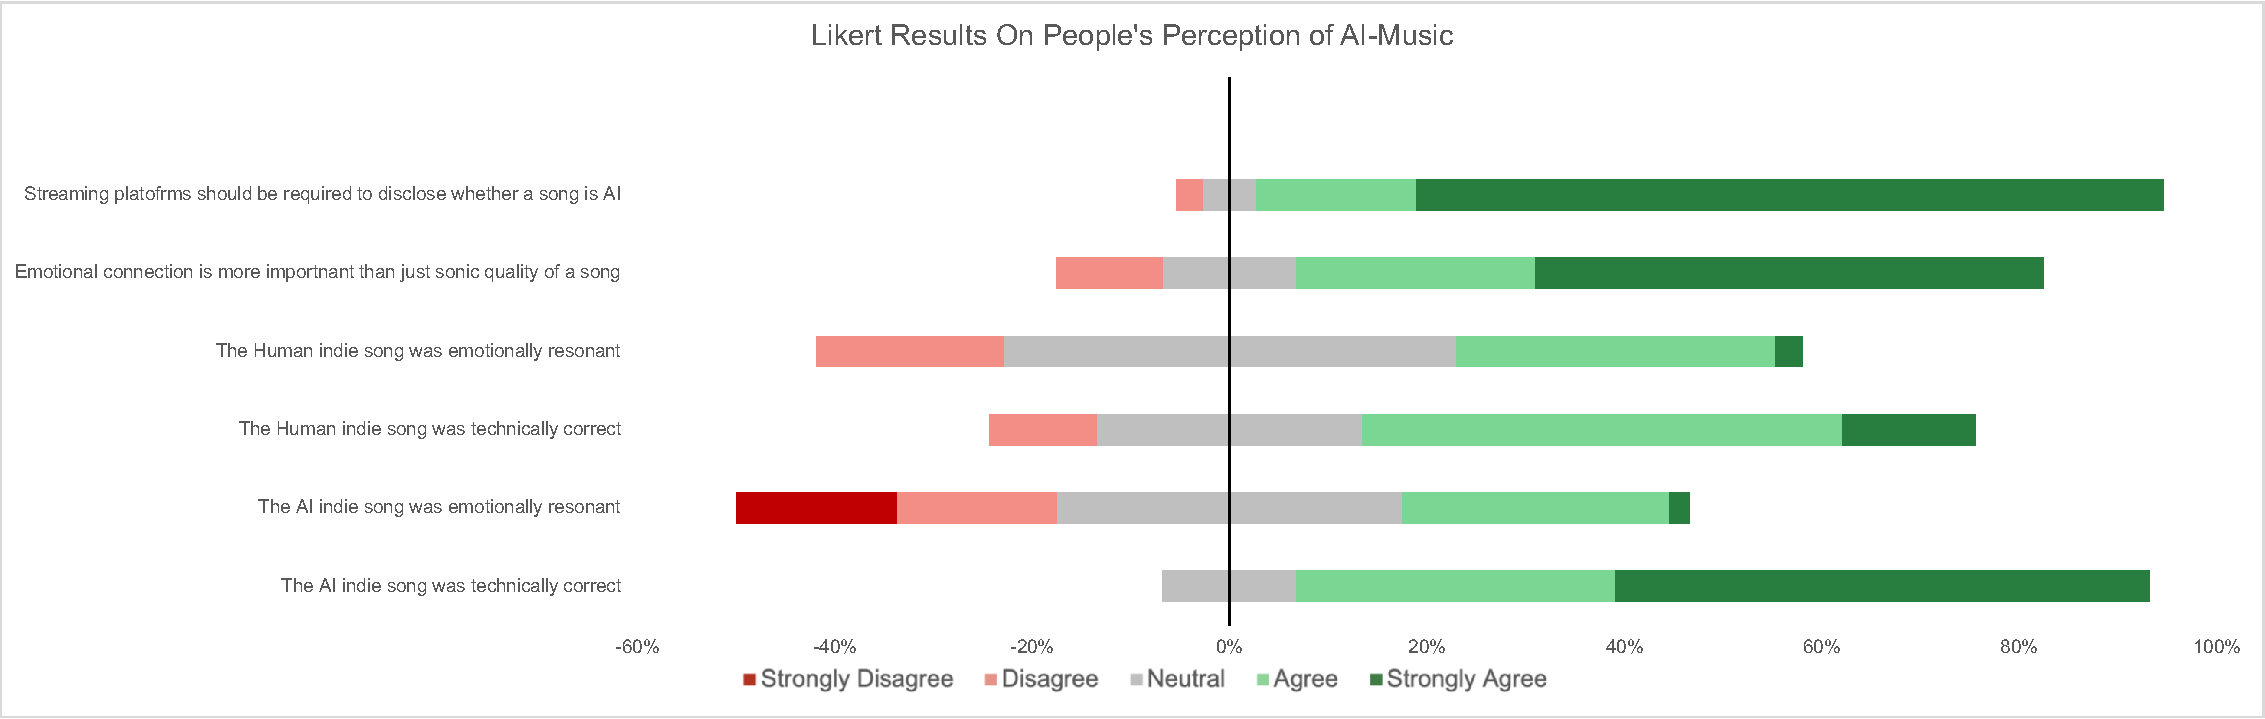
\includegraphics[width=1\textwidth]{Likert Results.pdf}
    \caption{Likert results from respondent perception of AI music }
    \label{fig:likert results}
\end{figure}


In terms of technical quality and production polish the AI track scored significantly higher, 86.5\%, compared to the human track, 62.1\% (see Figure \ref{fig:likert results}). This outcome was expected as AI models are trained on professionally mixed recordings spanning decades, giving them an advantage. A human producer working in limited time cannot compete with a model that has internalised the entire history of recorded music production.

However, technical quality did not translate into emotional engagement. When asked whether they felt an emotional connection to the music, 32.4\% of respondents disagreed in relation to the AI track, compared to only 18.9\% for the human track (see Figure \ref{fig:likert results}). Even when listeners could not explicitly identify which song was AI-generated (only 40.5\% guessed correctly, see Figure \ref{fig:comparison}), they still reported reduced emotional resonance with the AI output. When asked directly, 75.7\% of respondents agreed that ``my emotional connection to music comes from the artist's story, their emotions, and their live performance, not just the sound itself'' (see Figure \ref{fig:likert results}). This finding suggests that listeners' relationship with music is relational, not just sonic. People connect with music because they understand it as an expression of human experience, intention, and vulnerability. AI-generated music cannot fulfill this function because it has no lived experience.

\begin{figure}[h]
    \centering
    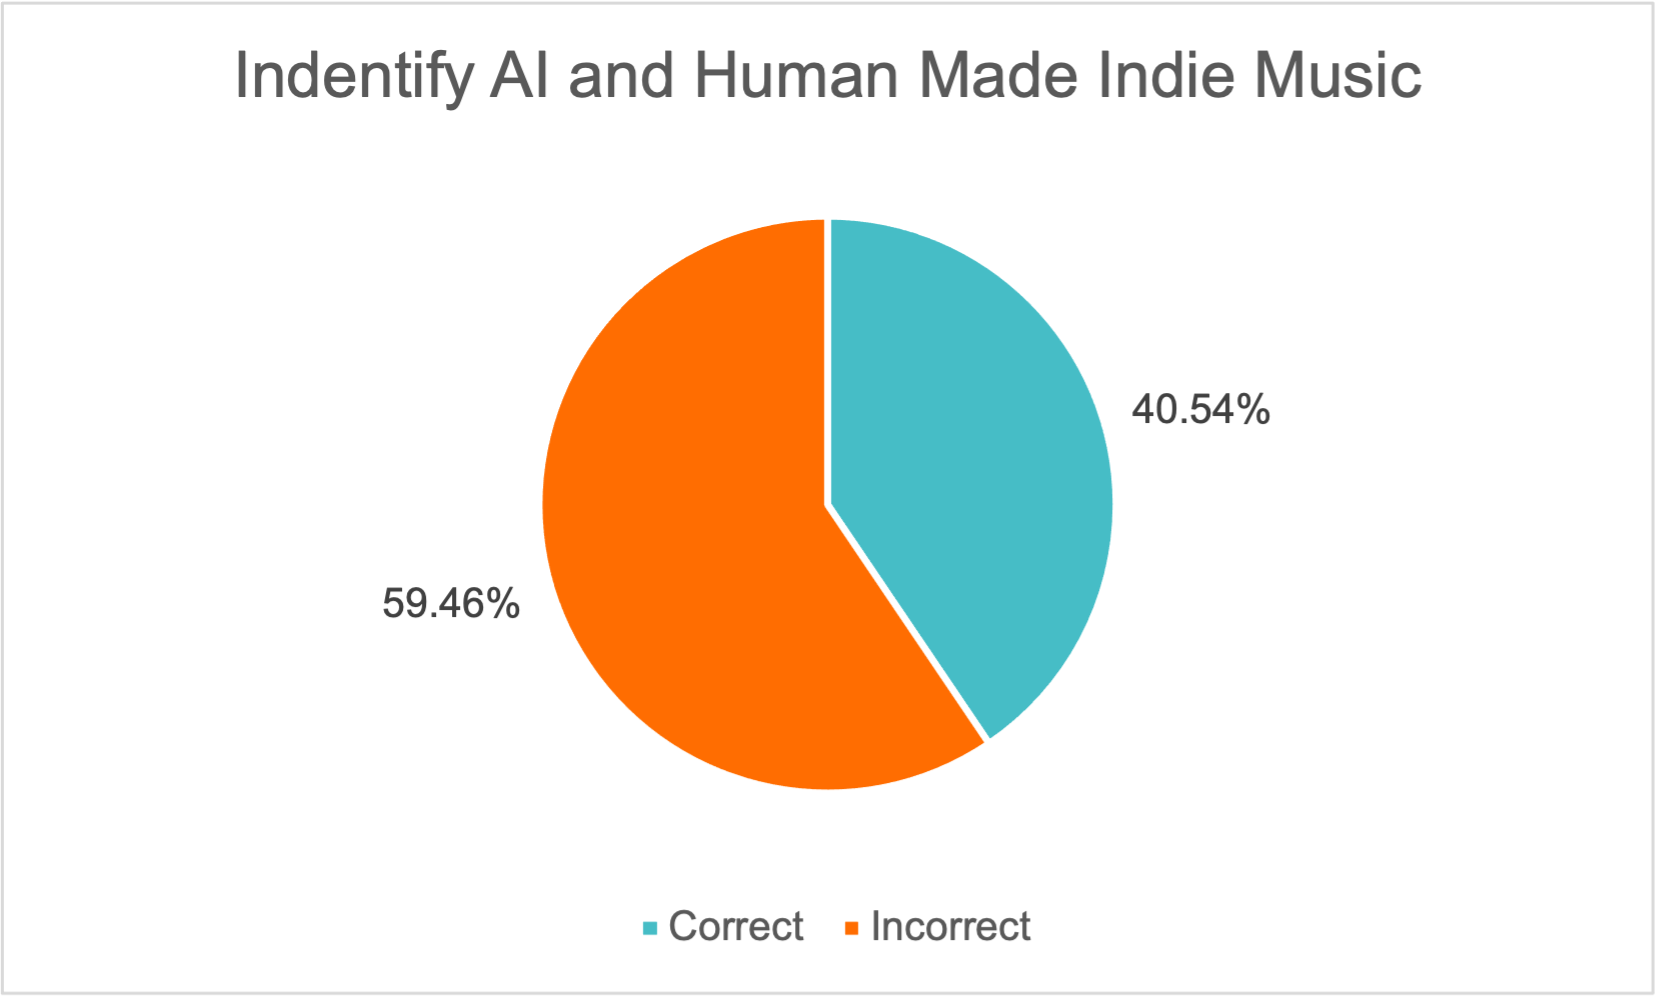
\includegraphics[width=0.49\textwidth]{Inide ID.png}
    \hfill
    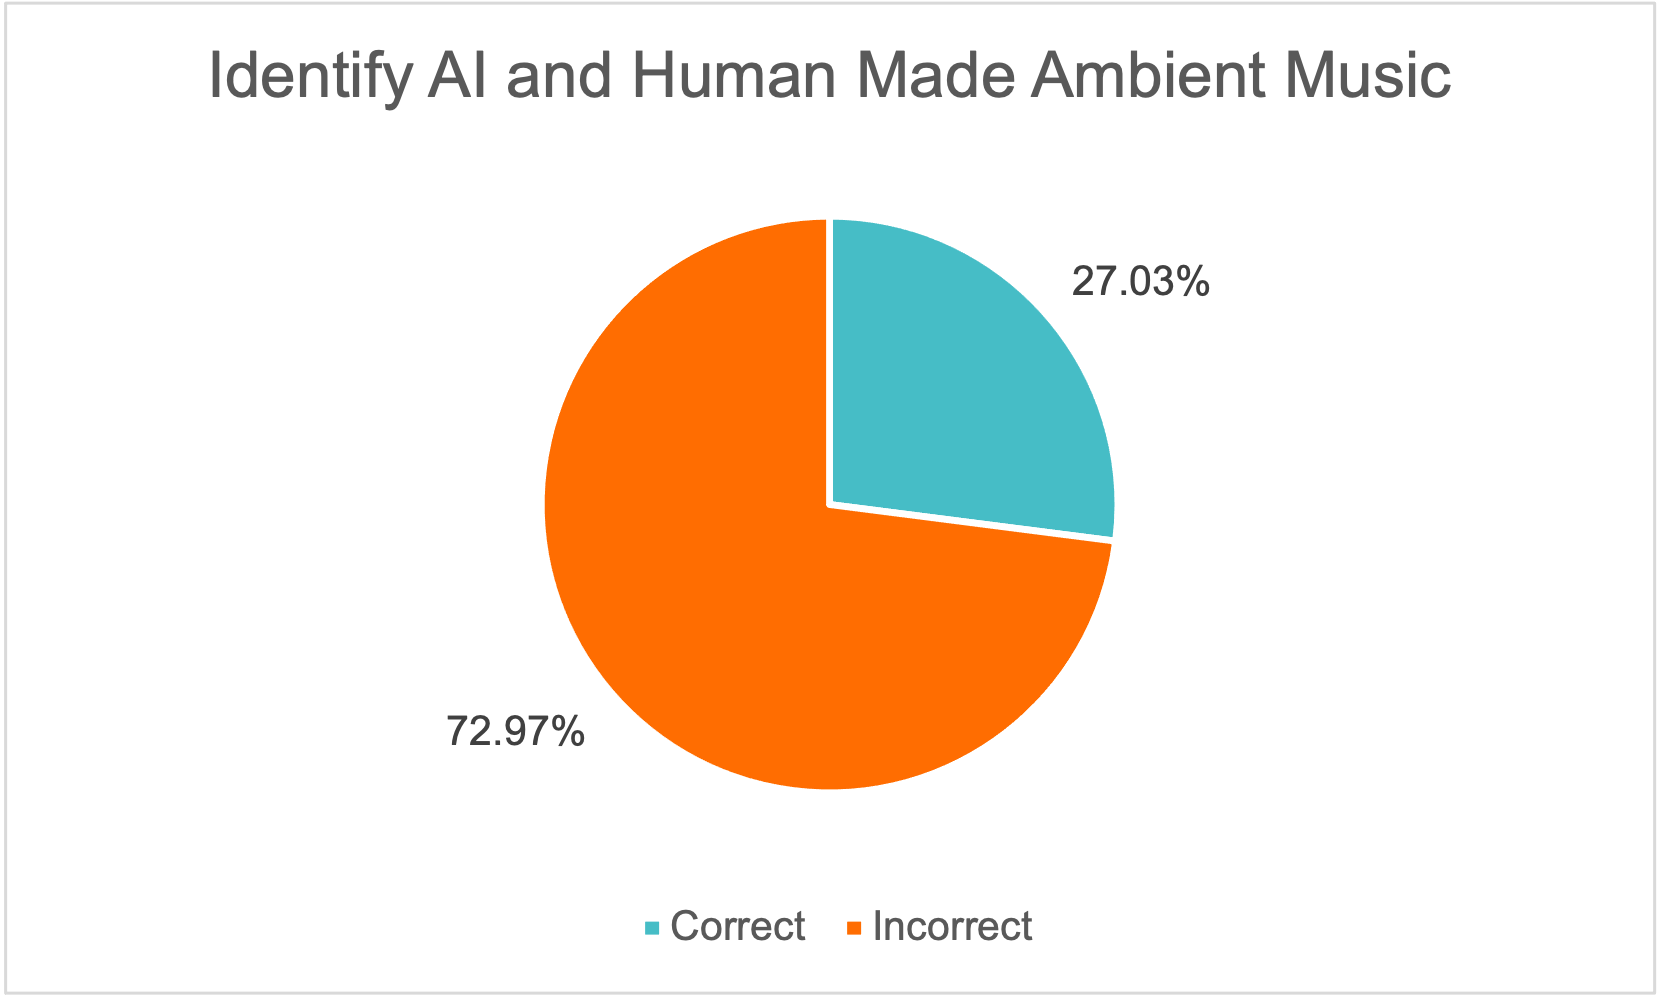
\includegraphics[width=0.49\textwidth]{Ambient ID.png}
    \caption{Results of identification success of AI music}
    \label{fig:comparison}
\end{figure}

This emotional disconnect translated into rejection of the music. Only 24.3\% of respondents said they would add an AI-generated song to their personal playlist. Many emphasised the lack of human element and emotional connection, arguing that music should reflect ``emotion, life experience, talent, effort, and creative artistry,'' which they perceived as absent in AI outputs. Others expressed support for human artists and ethical concerns, stating they wanted to support real musicians who dedicate years to developing their craft, rather than systems they viewed as ``stealing'' or ``imitating'' human work while ``reinforcing technofeudalism'' or ``killing an industry.'' Participants also questioned the nature of art and authenticity, with some describing AI music as not ``real'' art because it lacks ``meticulous craft, effort, or intention,'' calling it ``offensive'' or ``uncanny.'' Finally, respondents raised practical and philosophical reservations, noting that AI-generated music cannot be performed live, often sounds generic, carries environmental costs associated with AI training, and fails to provide the connection to known human artists that many listeners value.

One respondent captured this sentiment directly: \textit{``Not sure how I feel about music being made with AI. It is cool but I think it might take away the light and brilliance of how talented some people are with music. Also concerts are a major part of professional music and a way of people connecting to an artist. If a song is AI generated I would never be able to go see it live.''}

The survey's second phase tested ambient music, a genre designed for background utility rather than active emotional engagement. Participants listened to two ambient tracks generated from the prompt: ``Slow, deep, synth-driven, meditative and dreamy vibe, atmospheric with slow textures and nature sounds like birds and wind weaved in.'' Again, one track was generated by Suno and the other again composed by a human music producer. The results differed notably from the indie rock comparison. Only 27\% of respondents correctly identified the AI-generated ambient track, compared with the 40.54\% who correctly identified the Indie Rock track. This suggests that AI systems are more convincing in genres that do not rely on vocal performance or personal narrative (see Figure \ref{fig:comparison}). 

Acceptance of AI-generated music increased substantially in utility contexts. When asked whether they would be comfortable with the AI ambient track being used at a meditation retreat, 59\% responded affirmatively. This contrasts with the 24.3\% willing to add an AI-generated indie song to their personal playlist (see Figure \ref{fig:likert results}). When asked directly about contexts in which they would be comfortable listening to AI-generated music, a clear pattern emerged: respondents accepted AI music for background purposes (59.5\%), advertisements (51.4\%), and video games or movies (45.9\%), but overwhelmingly rejected it for active/focused listening (8.1\%). Only 16.2\% found AI music acceptable for social events like parties or dinners, and 35.1\% stated they were not comfortable with AI-generated music for any purpose (see Figure \ref{fig:acceptance}).

\begin{figure}[h]
    \centering
    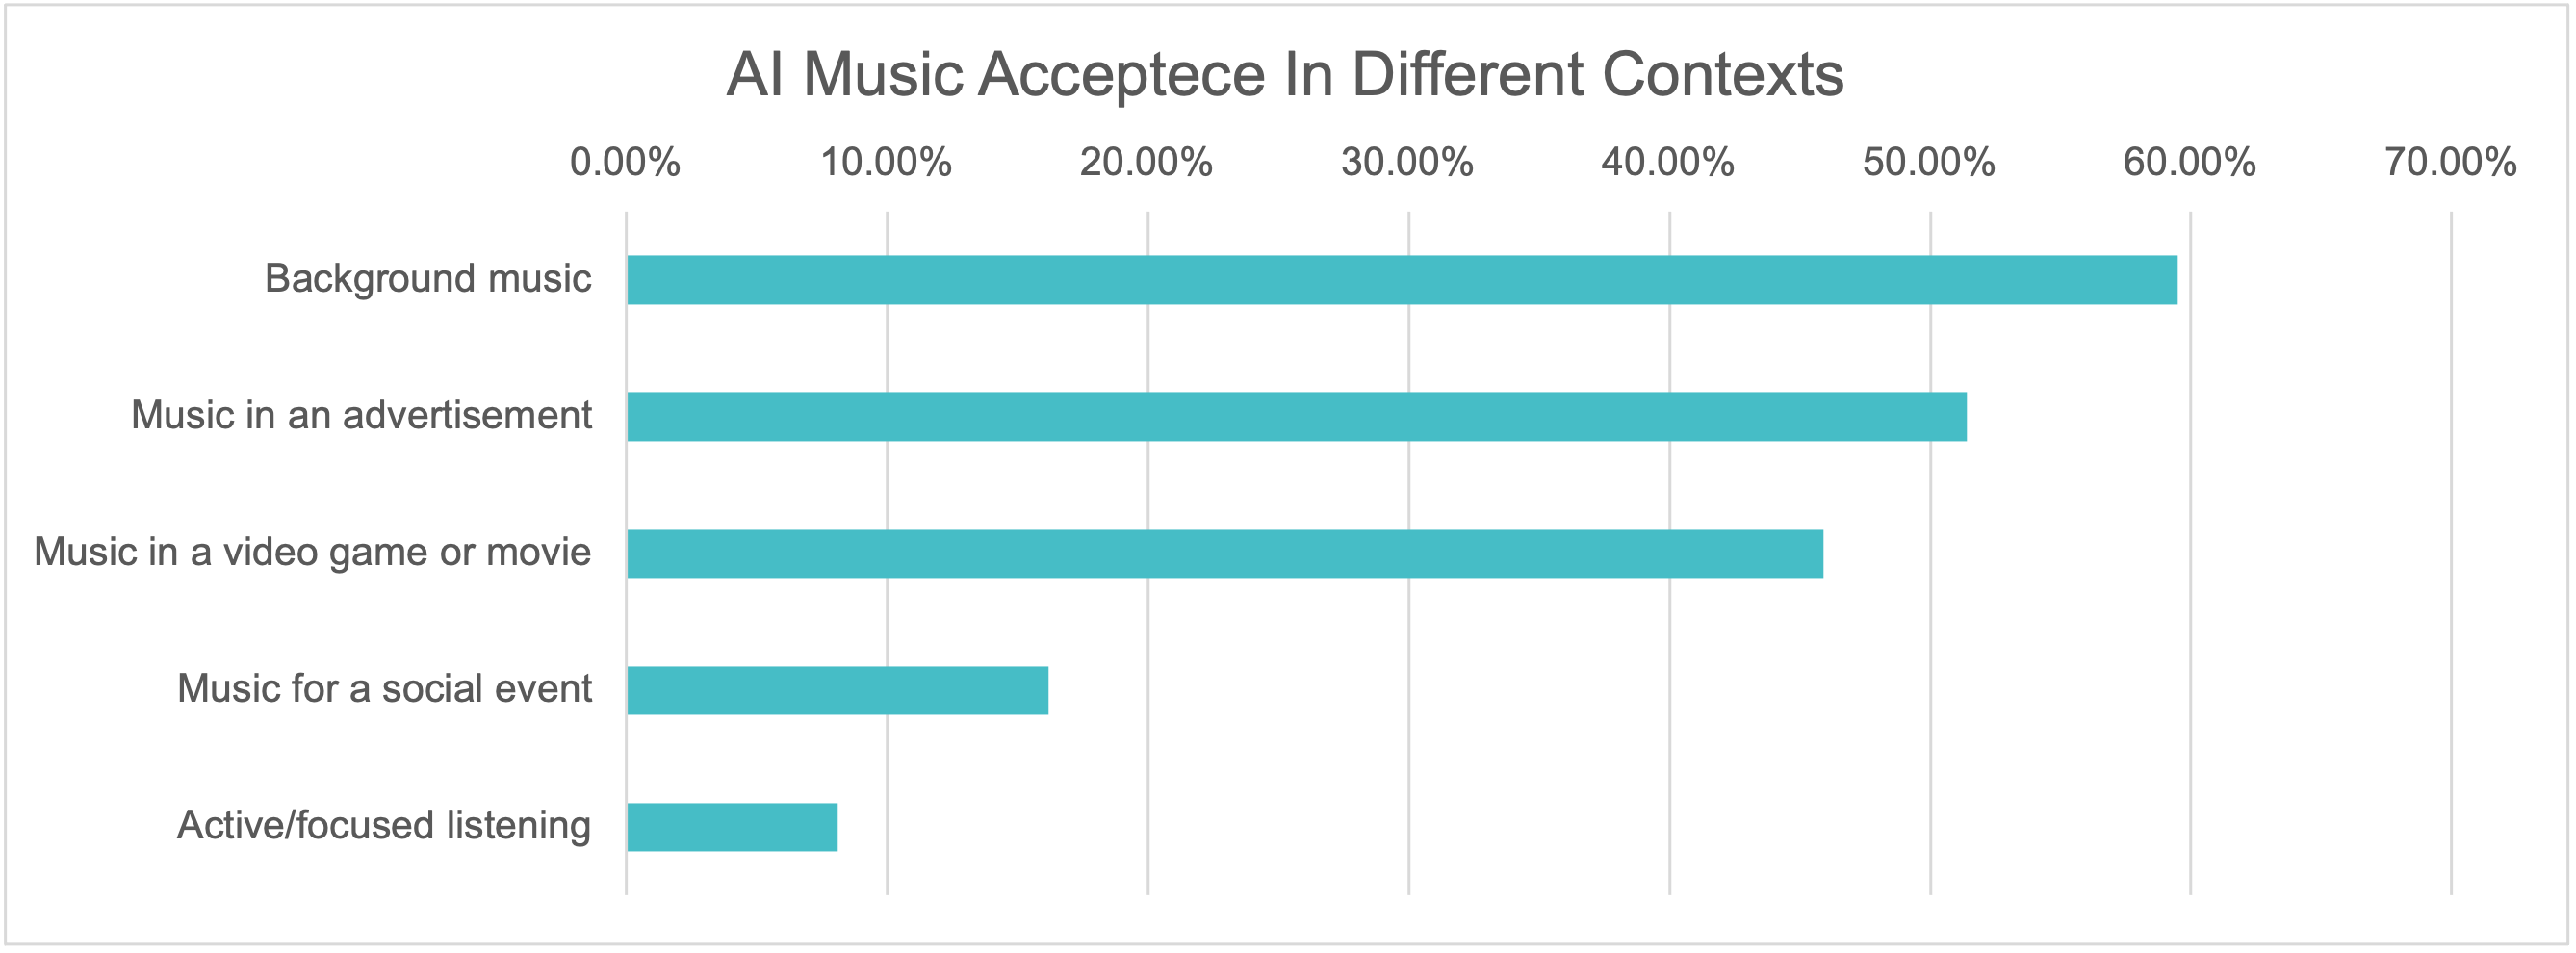
\includegraphics[width=1\textwidth]{Acceptance in context.png}
    \caption{Acceptance of AI music in different contexts}
    \label{fig:acceptance}
\end{figure}

This pattern in consumer acceptance suggests a likely future trajectory, AI-generated music will establish dominance in commercial and utility contexts where music functions as atmosphere, while human musicians will continue to dominate in artistic and personal listening contexts where emotional connection and authenticity matter. This however, would represent a significant reduction of professional opportunities for human musicians, particularly those working in commercial music production for advertising, games, film, and content creation. These sectors have historically provided stable income for working musicians who may not achieve mainstream recognition but rely on licensing and commission work to sustain their careers. If AI systems capture these markets, the economic foundation supporting a diverse musical ecosystem erodes, potentially funneling the music industry toward a model where only artists capable of fostering an engaged fan-base are able to achieve success.

Another finding from the survey was the demand for transparency. When asked whether streaming platforms should be required to label AI-generated music, 91.1\% of respondents agreed (see Figure \ref{fig:likert results}). Many participants expressed feeling deceived when they were not informed whether a song was AI-generated, viewing the lack of disclosure as a violation of trust. This aligns with broader patterns in consumer attitudes toward AI systems: people want to know when they are interacting with algorithmic outputs rather than human-created content, and they view non-disclosure as misleading.

\section{Conclusion}

The future of AI-generated music is far from predetermined. The technology will continue to improve, and its commercial presence will likely expand. However, whether AI music becomes a legitimate and sustainable component of our musical culture depends entirely on the regulation, ethical considerations, and the consumer sentiment that emerges over the next few years.

If current practices continue, such as unauthorised training on copyrighted material, copyright protection for purely algorithmic outputs, recursive training leading to model collapse, and cultural appropriation of Indigenous music, AI-generated music will function as an extractive technology that displaces human musicians, homogenizes musical culture, and funnels economic power to a small number of AI companies. 

The ethical baseline is clear: explicit permission and compensation for training data, no copyright for prompt-only outputs, prevention of model collapse through dataset curation, and genuine respect for Indigenous cultural sovereignty. The survey also unveiled some consistent patterns in the consumer landscape: people accept AI music for utility but reject it for personal connection. People also want to know if what they are listening to is AI-generated. These two conclusions define the boundaries within which AI music can operate sustainably. Companies that refuse to meet these standards should face regulatory consequences and platforms that flood the market with unlabeled AI content should be held accountable for undermining transparency and consumer trust.

Music is one of the purest forms of human expression and should be treated as such. If AI music systems are to exist within this space, they must do so in ways that protect and amplify human creativity rather than displace it. The technology is here, the question is whether we will deploy it with thoughtful intention.
    


\bibliographystyle{IEEEtran}
\bibliography{sample}

\end{document}
